\chapter{The CMS Detector}
\label{chap:detector}

To ensure as much as possible of the debris of the proton-proton collisions can be detected, CMS is constructed to maximize the solid-angle coverage of the interaction region. The 20$\,$cm transverse size of the beam-pipe prohibits instrumentation in the most forward of this region. CMS is composed of a modular design of different detectors, each with their own technology and working points, allowing for direct measurements of a wide spectra of particles. Figure \ref{fig:howcmsworks} illustrates how well instrumented the interaction region is, highlighting each of the detector systems. The proton-proton beamline is seen as a grey tube oriented from the bottom right to the top left of the figure. The interaction region is within the silicon tracker.

Only the lightest particles within the SM have a long enough lifetime to travel any appreciable distance within our detector. Electrons $e^{\pm}$, photons $\gamma$, and protons $p^{\pm}$ are stable and can be directly detected via interactions with the bulk of the detector. Muons $\mu^{\pm}$, pions $\pi^{\pm}, \pi^{0}$, neutrons n, and kaons $K^{\pm}, K^{0}$ are intrinsically unstable but have long enough lifetimes to travel far enough to interact with our detector. The different CMS subdetectors responsible for the detection of these particles are seen in Figure \ref{fig:schematicview}. By piecing together these elements we are able to provide a reconstruction of the physics processes occurring within each particle collision. Different types of interactions leave unique signatures by decaying into specific final states, which are those we detect. We can not directly detect neutrinos $\nu$, but must infer there presence from an imbalance in the total momentum of the event; precision neutrinos physics requires specialized detector technology.

The detector can generically be divided into central \textit{barrel} and forward \textit{endcap} regions. The geometry either takes the form of concentric cylinders (in the barrel) or flat planes of detectors (in the endcaps). Figure \ref{fig:detectoreta} illustrates these barrel ($|\eta|<1.5$) and endcap ($1.5<|\eta|<5$) regions. The beamline is seen as the thin cyan line across the base of the image.  

This chapter will discuss the main elements of the CMS detector, beginning with the innermost (closest to the beam pipe) silicon tracker and concluding with the muon tracker. 

\begin{figure}[hb!]
\centering
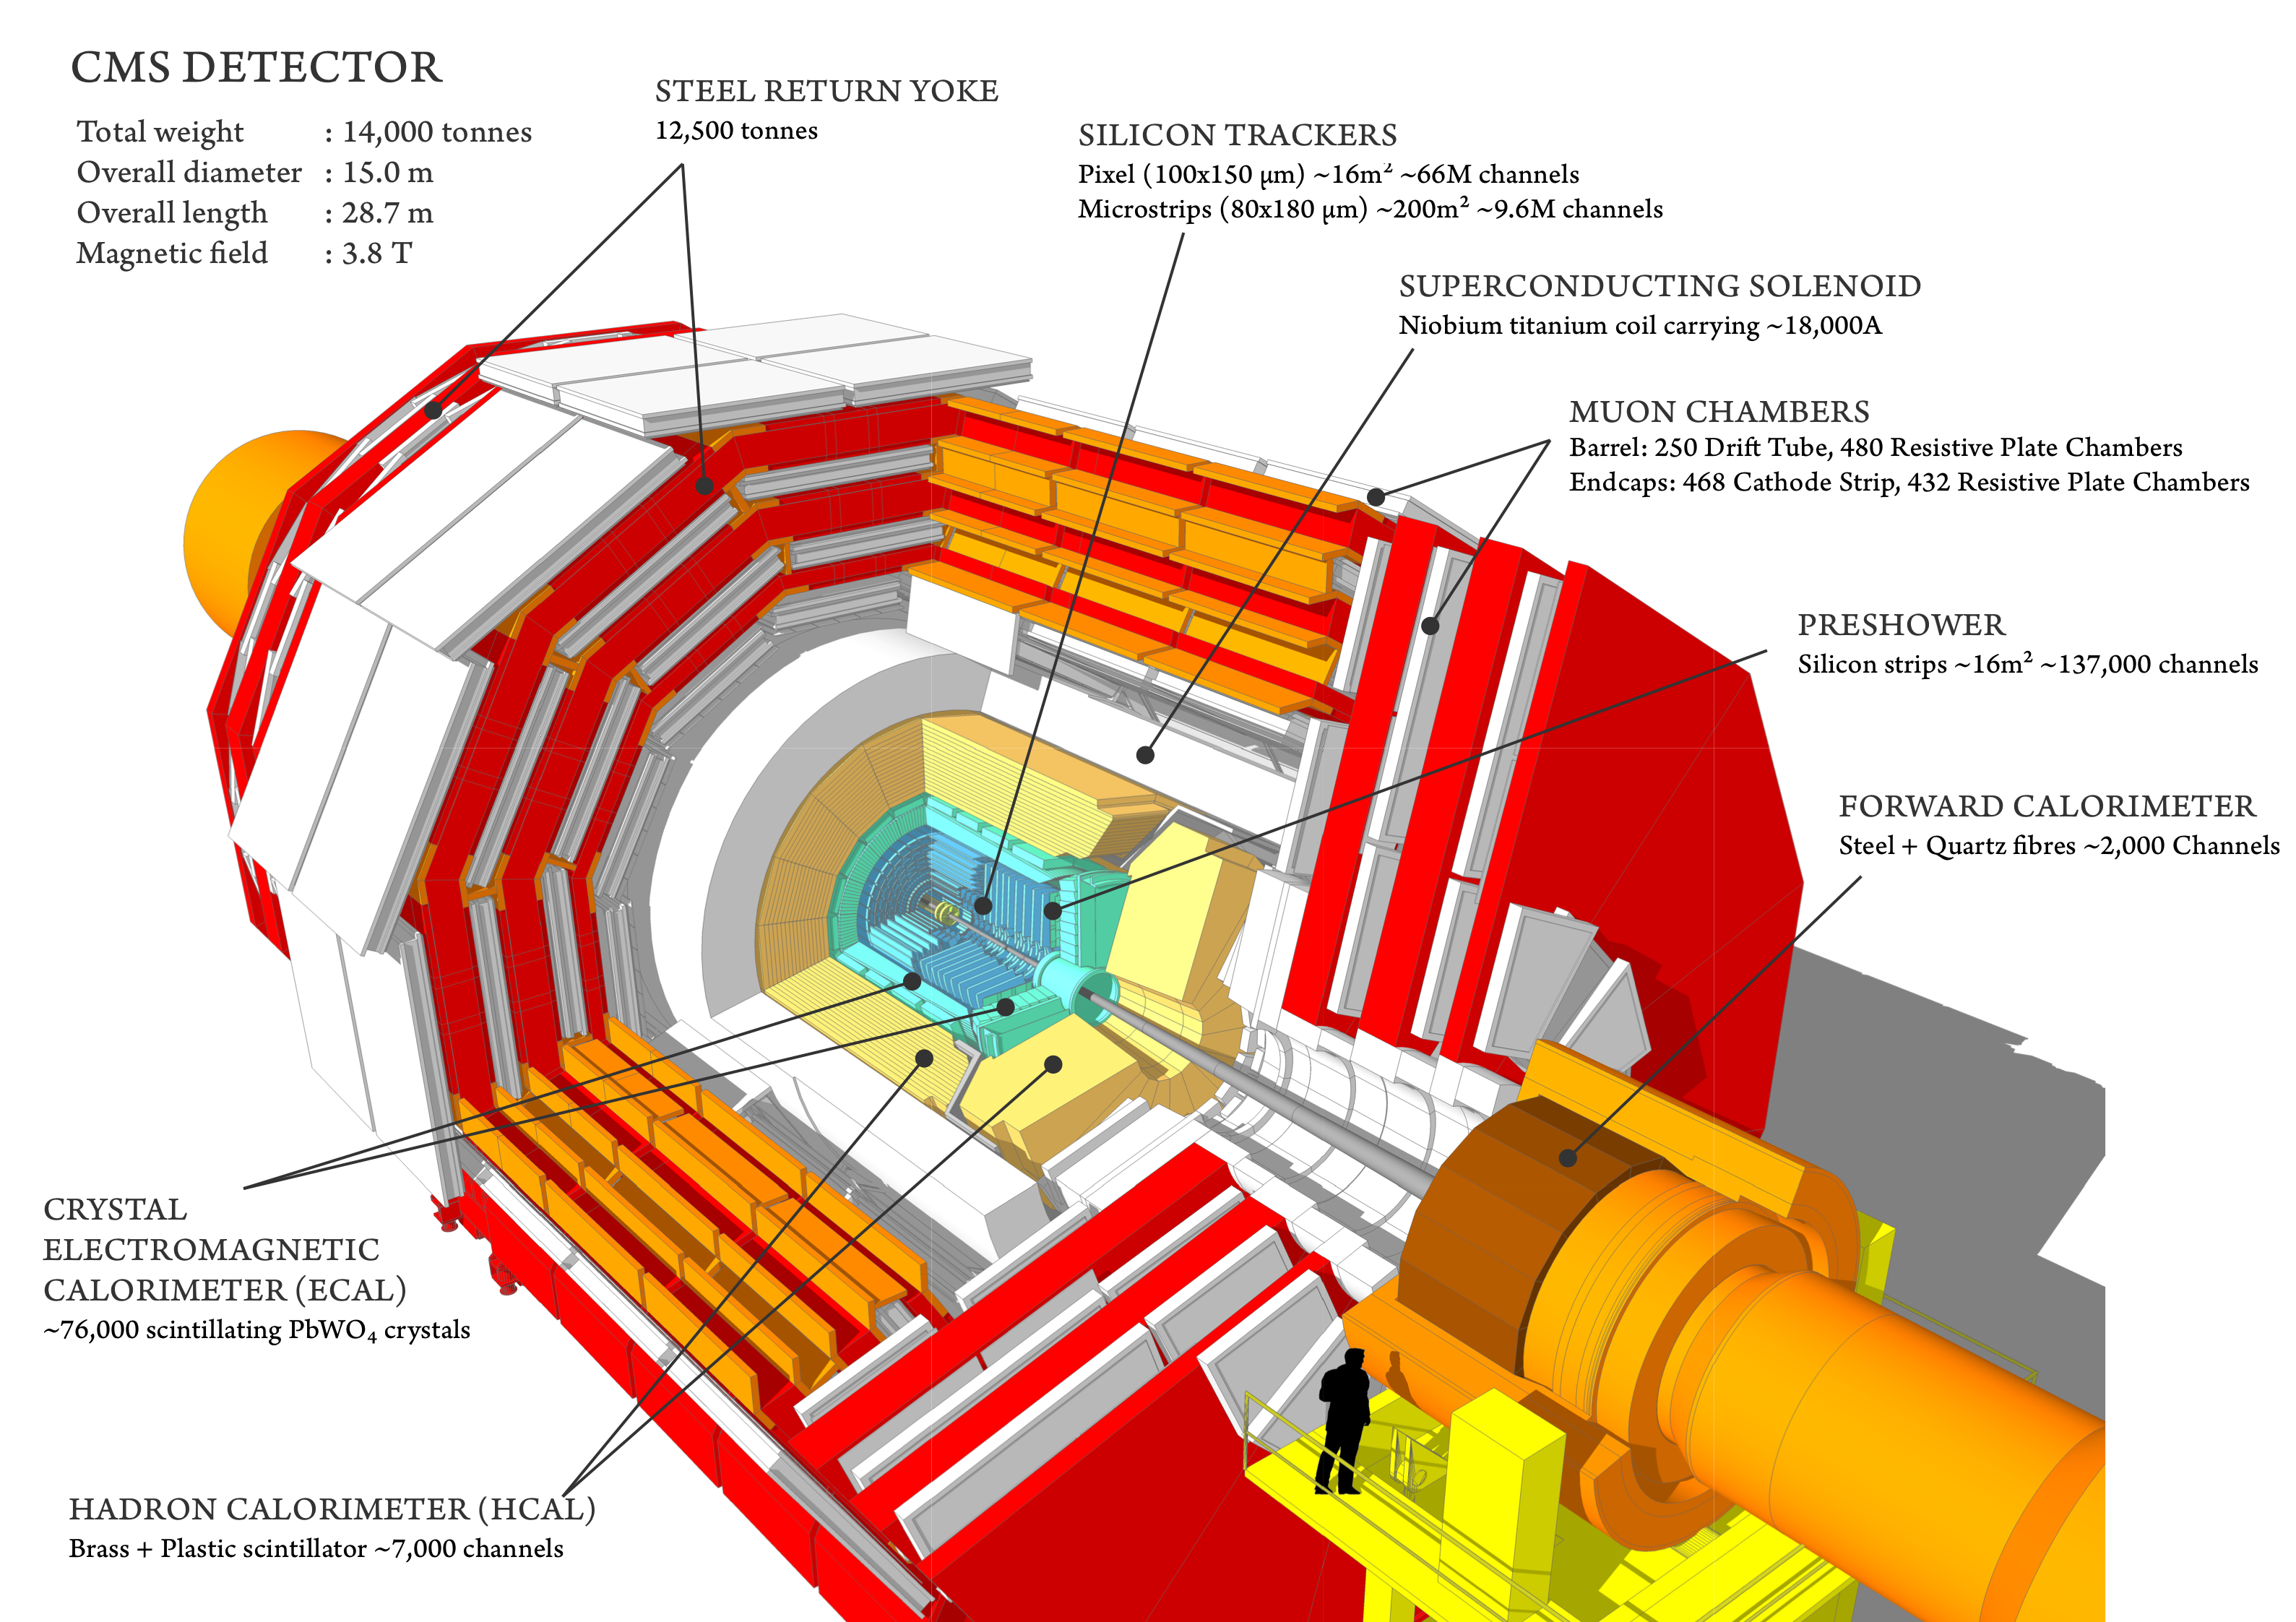
\includegraphics[width=0.9\textwidth]{figs/howcmsworks.png}
\caption{A diagram of the CMS detector. Detector subsystems are labeled.}
\label{fig:howcmsworks}
\end{figure}

\begin{figure}[hb!]
\centering
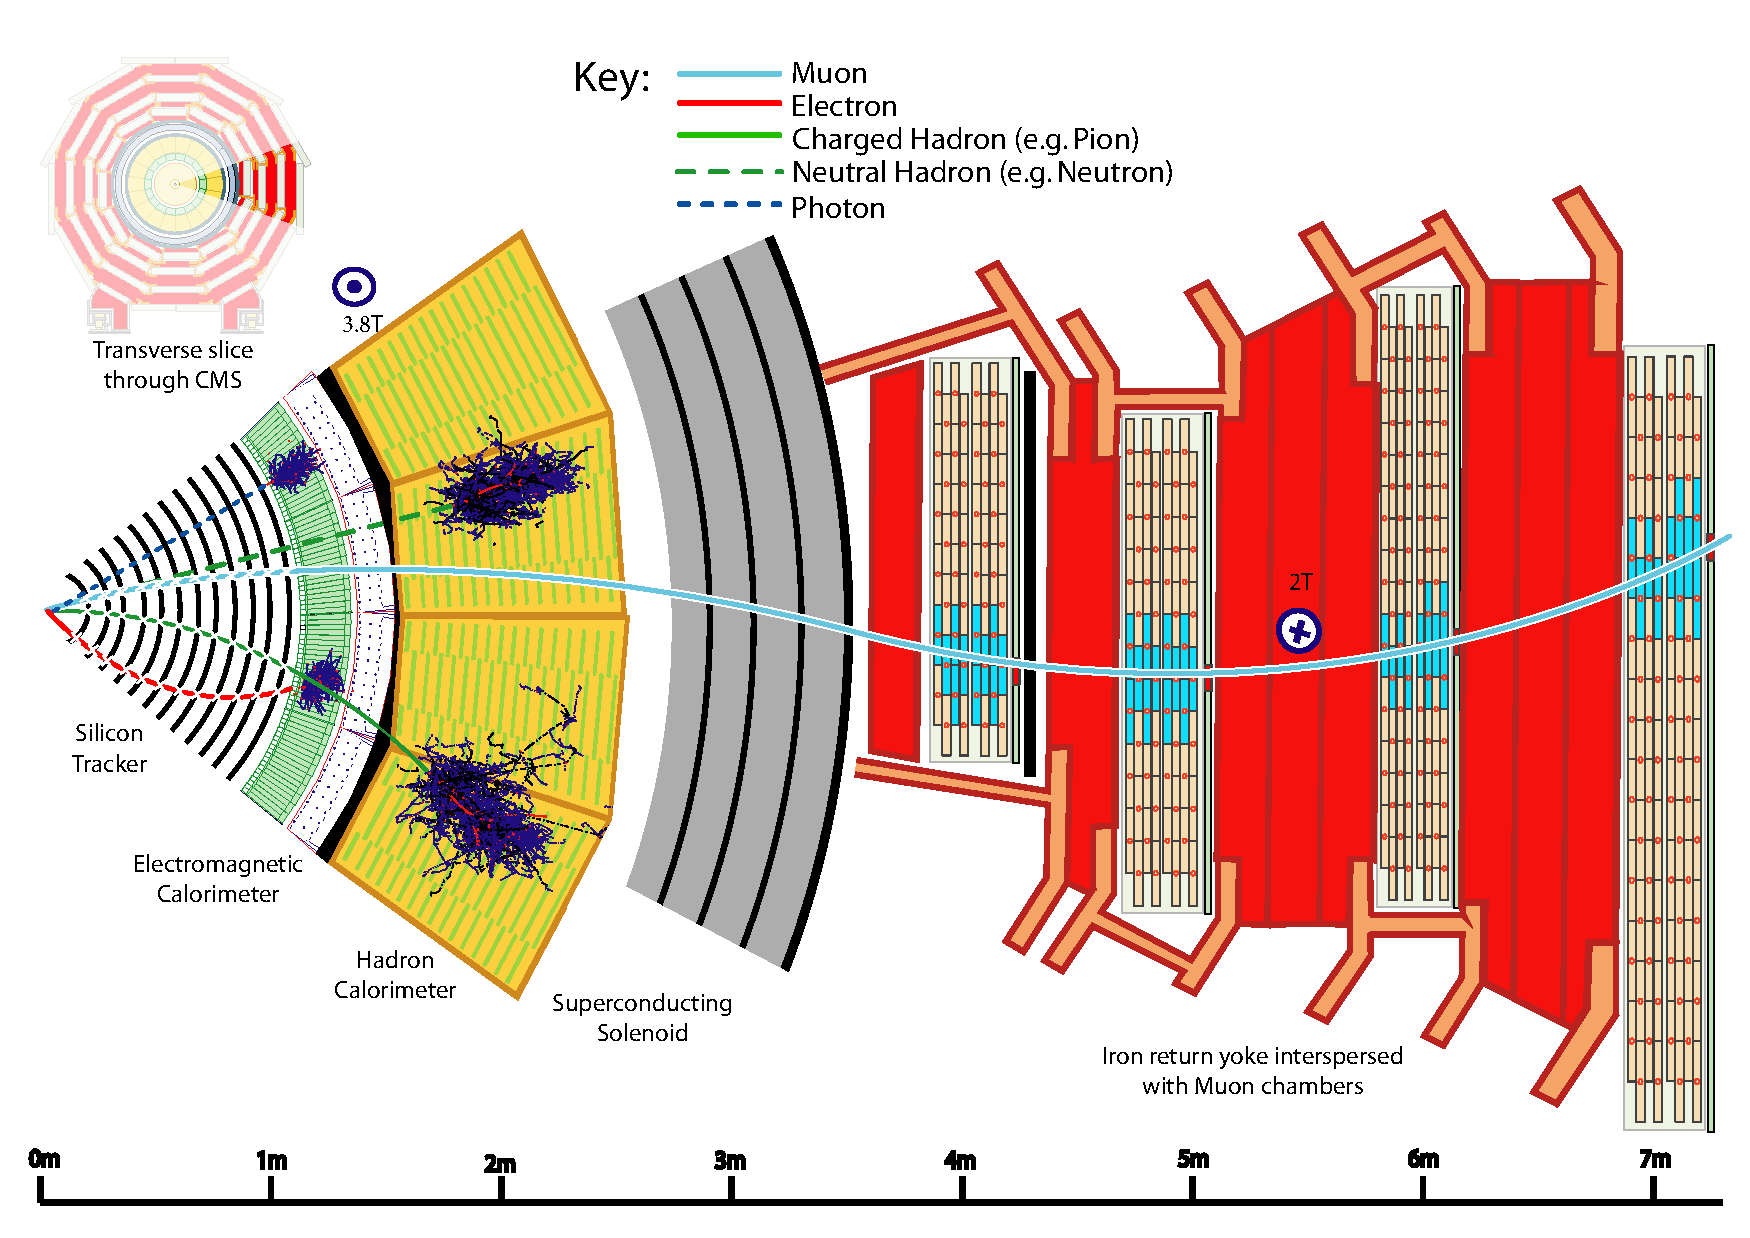
\includegraphics[width=0.875\textwidth]{figs/CMS-PRF-14-001_Figure_001.pdf}
\caption{A diagram of the CMS detector in the r-$\phi$ plane; the beam axis is perpendicular to the page. SM particle signatures within the detector are shown.}
\label{fig:schematicview}
\end{figure}

\begin{figure}[hb!]
\centering
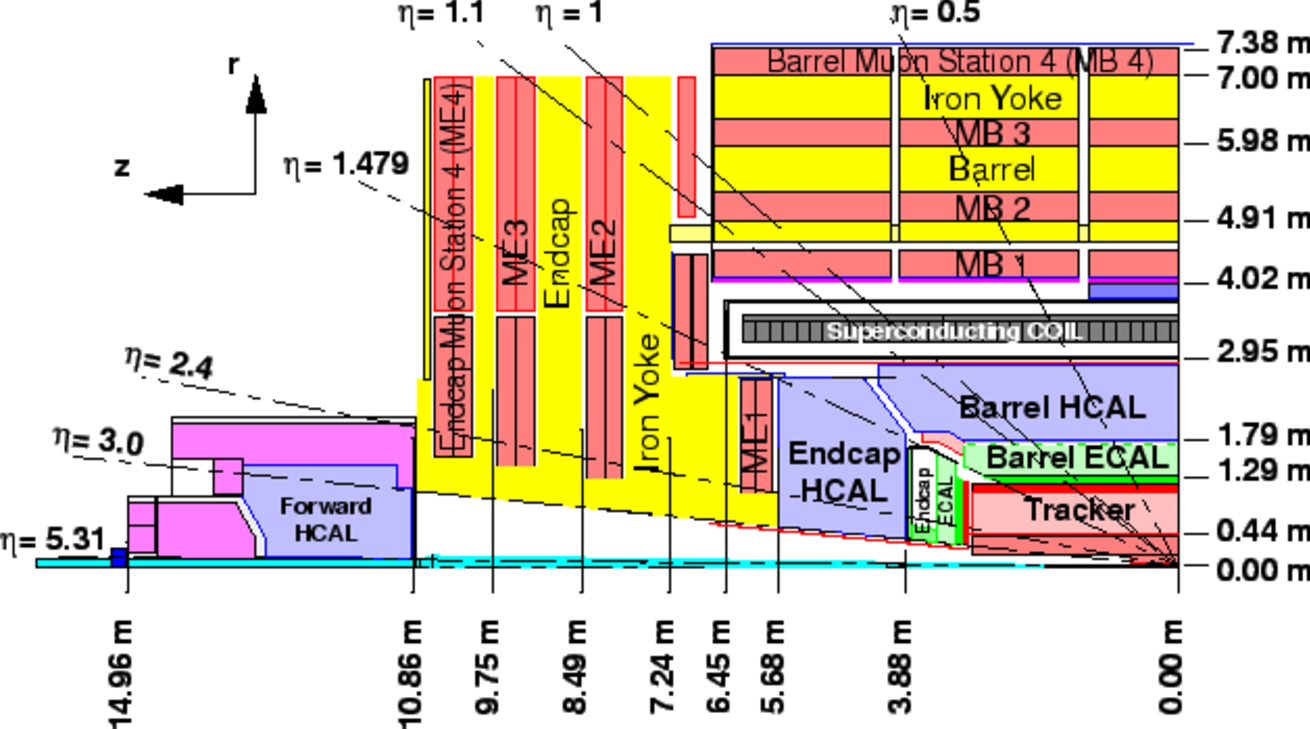
\includegraphics[width=0.8\textwidth]{figs/img41.pdf}
\caption{A diagram of the CMS detector in the r-z plane; the beampipe is the thin cyan sliver along the bottom. The detector subtends a large solid angle about the interaction region.}
\label{fig:detectoreta}
\end{figure}

\section{Silicon Tracker}

The silicon tracker is responsible for the reconstruction of charged particles: electrons, muons, kaons and pions. The particle trajectory is reconstructed using ionization deposits left in layers of thin silicon. The particle momentum is measured by the curvature of the trajectory when submerged in the magnetic field.\cite{trackertdr} \cite{trackertdradd}

The tracker is built of modules consisting of a layer of sensitive silicon bonded on top readout electronics. The silicon is arranged as a p-n junction, reversed-biased and fully-depleted. As a charged particle travels through the material, it ionizes the silicon creating electron-hole pairs within the depletion zone. Electric fields accelerate the charge through the silicon to the readout electronics bonded to the back of the sensor. The readout chips amplify, digitize, and store the hit information before being piped outside the detector. The silicon is very thin (~300$\mu$m), the tracker is constructed of as little material as possible so as not to perturb the trajectory of the particle.

The silicon tracker is divided into two major components. The pixel detector is at a closer proximity to the beam line and has finer spatial segmentation. The strips detector covers a much larger spatial volume and is responsible for the majority of the hits along a particle trajectory. A diagram of the geometry and layers of the tracker is seen in Figure \ref{fig:tracker}.

\begin{figure}[hb!]
\centering
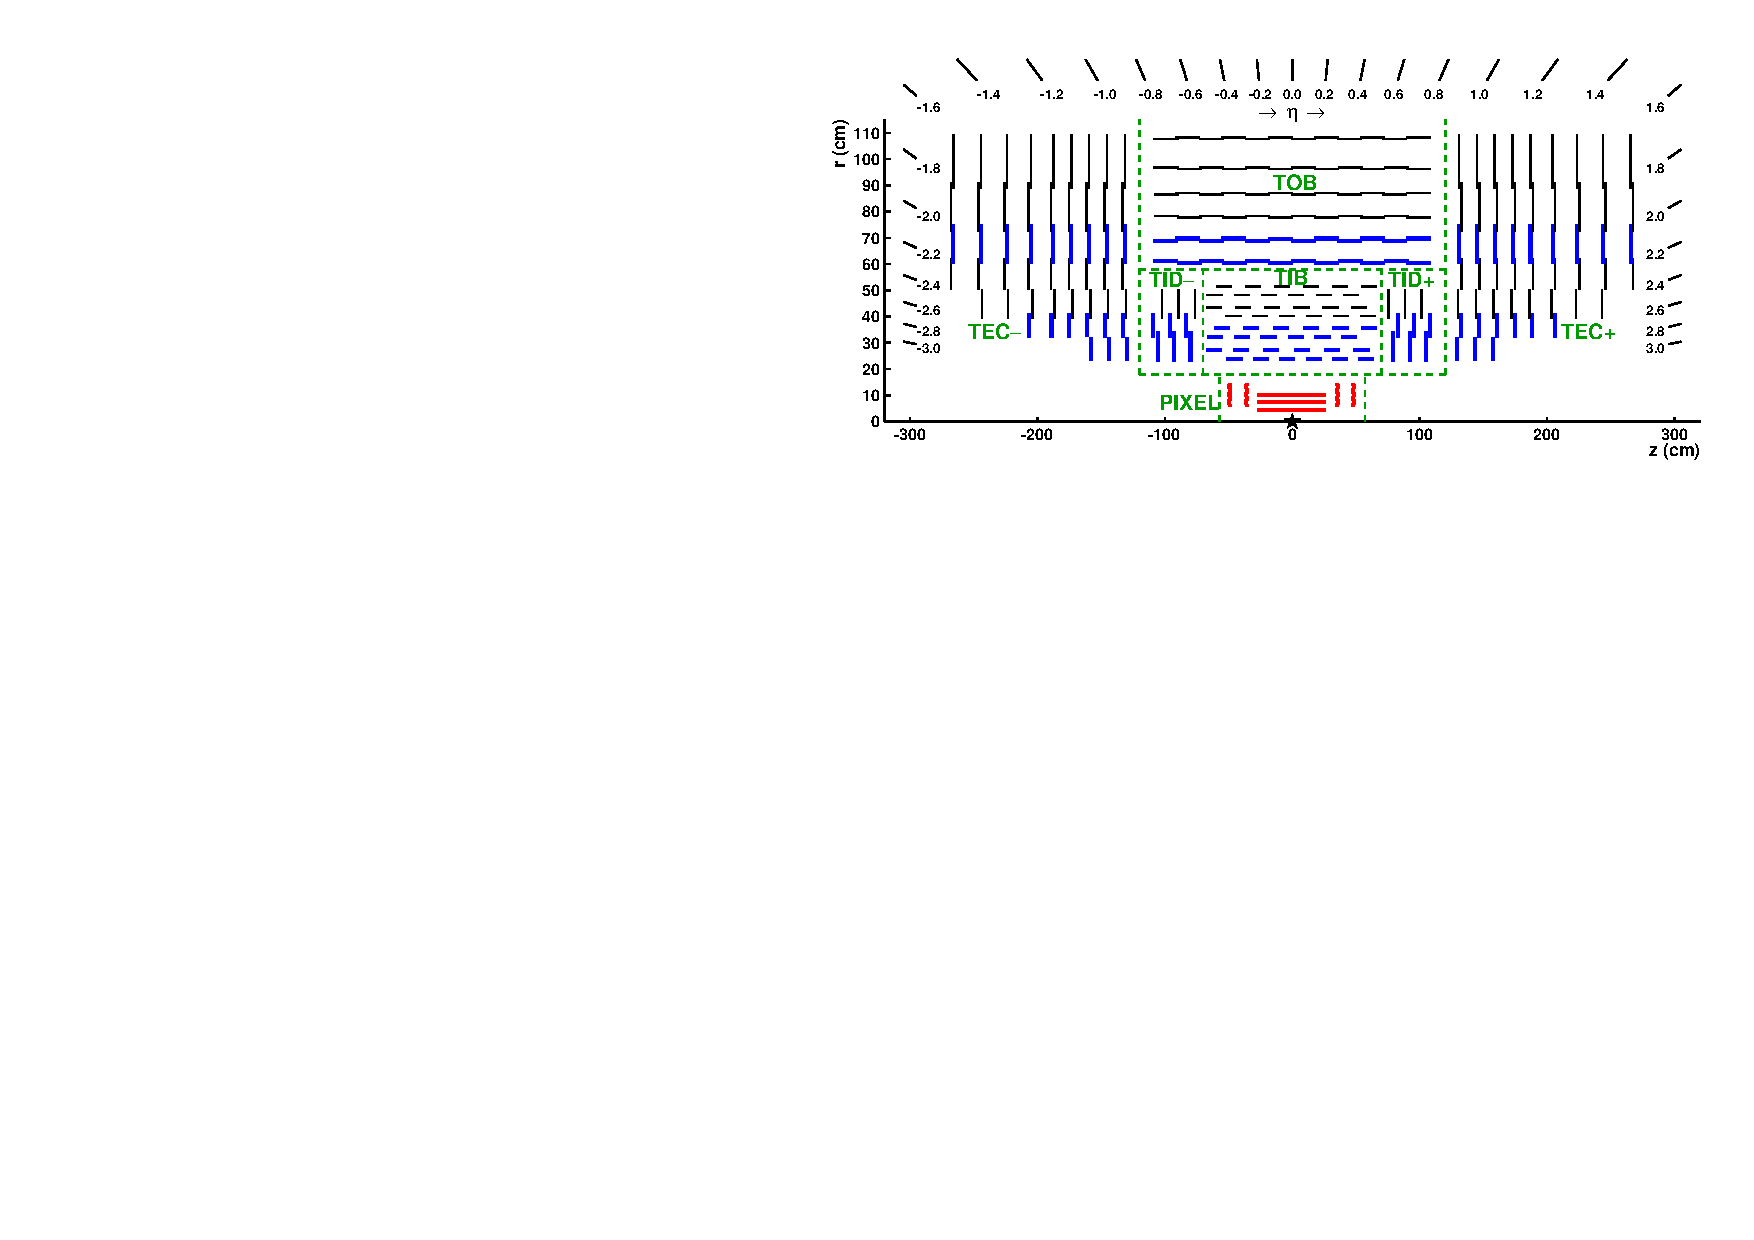
\includegraphics[width=0.8\textwidth]{figs/TrackerLayoutNew.pdf}
\caption{The CMS silicon tracker. The vertical and horizontal lines represent layers of silicon modules.}
\label{fig:tracker}
\end{figure}

\subsection{Pixel Detector}

The task of the pixel detector is to provide the spatial granularity required for precision track vertexing. The barrel region ($|\eta|<1.5$) of the pixel detector consists of 4 concentric cylinders sitting at radii between 2.9 and 16 cm from the beamline. The endcaps ($1.5<|\eta|<2.5$) consist of three discs on each side ($\pm$z) placed in between z = 3.2 and 4.8cm. The pixel size on the silicon modules is 100x150$\mu\,m$ wide, consisting over of 65 million channels in total.

\subsection{Strips Detector}

The silicon strips detector sits immediately outside the pixel detector and provides additional hits along a particle's trajectory: the barrel region ($|\eta|<1.5$) provides 10 layers, the endcaps ($1.5<|\eta|<2.5$) provide 12. The silicon modules are partitioned in strips ranging from $80-180\,\mu$m wide, yielding more than 10 million individual readout channels.

\section{Electromagnetic Calorimeter}

The electromagnetic calorimeter is responsible for the reconstruction of electrons $e^{\pm}$, photons $\gamma$ and charged pions $\pi^{\pm}$. The energy is measured by collecting the light generated by an electromagnetic shower as the particle is absorbed in the calorimeter.\cite{ecaltdr}\cite{ecaltdradd}

The bulk of the calorimeter consists of lead-tungstate (PbWO$_{4}$) crystal. Electromagnetic showers are created when high energy particle enters the material. Low-mass particles, such as electrons, scatter as they traverse the material and emit bremstrallung radiation in the form of lower-energy photons. Photons interact with the material and convert into an electron-positron pair, which themselves are able to then emit radiation. The light generated by this shower is collected using photodetectors mounted at the end of each crystal. Light incident on the photodetector first encounters silicon where the photon knocks an electron of a silicon atom. This electron is accelerated with an electric field onto an electrode surface which liberates electrons via the photoelectric effect. These electrons are accelerated onto another electrode which in turn liberate more electrons. This signal is then further amplified and digitized.

The electromagnetic calorimeter is divided into barrel ($|\eta|<1.5$) and endcap ($1.5<|\eta|<3$) regions comprising over 75,000 crystals. The crystals measure 2.2$\,$x$\,$2.2$\,$x$\,$23$\,$cm in the barrel (matching the Moliere radius of PbWO$_{4}$ - 2.2 cm) and 3$\,$x$\,$3$\,$x$\,$22$\,$cm in the endcaps; they are oriented radially outward from the interaction region. A schematic of the detector is seen in Figure \ref{fig:ecal}. This thickness of absorber is sufficient to contain over 98\% of the energy of incident particles. Additionally, the electromagnetic calorimeter serves as an absorber for the hadronic calorimeter, initiating a shower in approximately 1/3 the particles headed for the hadronic calorimeter.

\begin{figure}[hb!]
\centering
\begin{subfigure}[b]{0.35\textwidth}
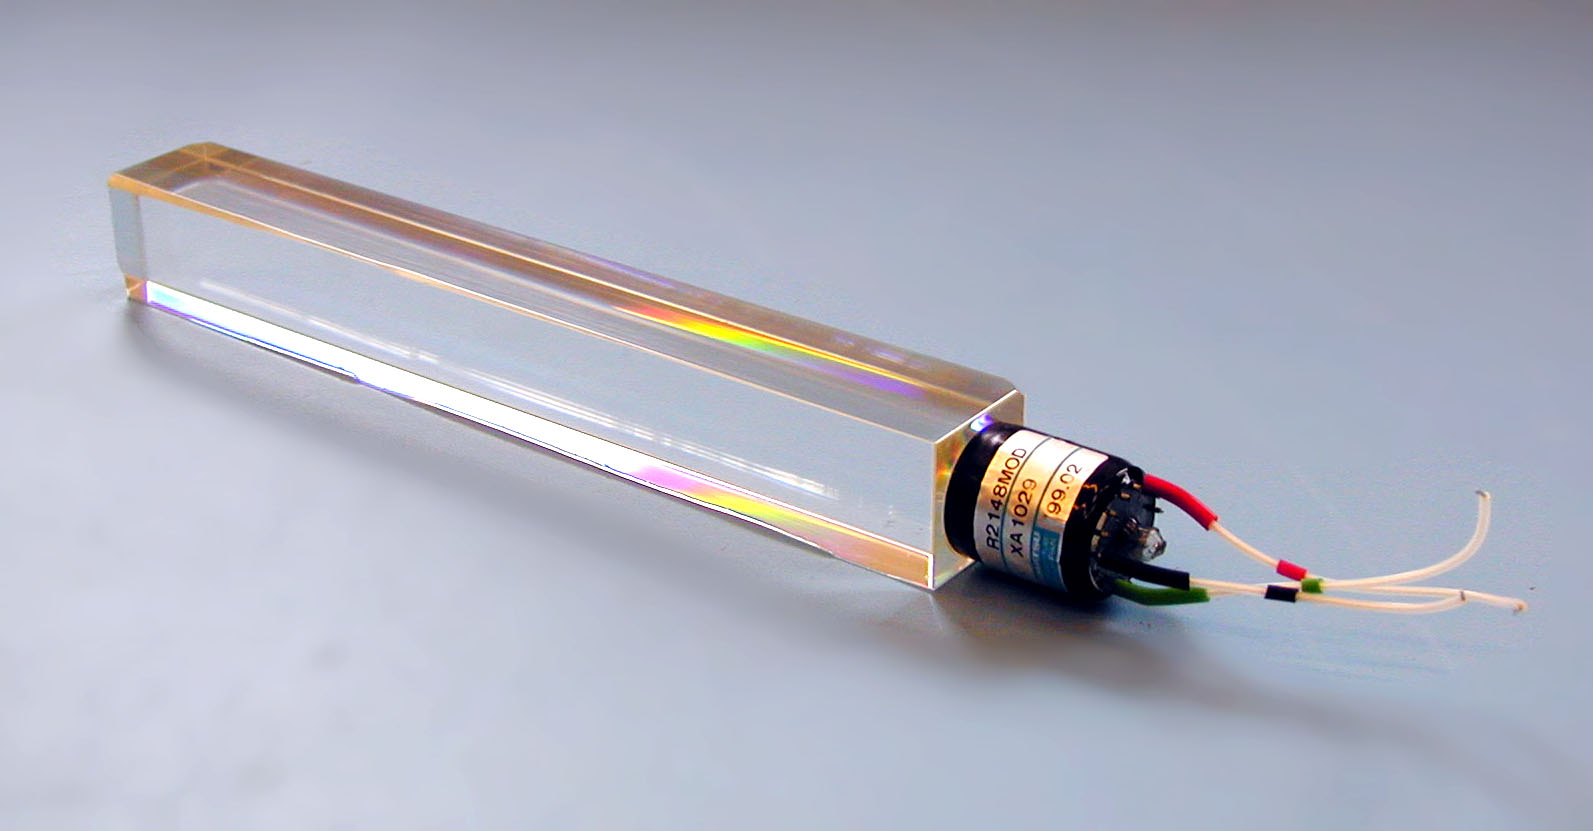
\includegraphics[width=\textwidth]{figs/ecalcrystal.jpg}
\caption{A single PbWO$_{4}$ crystal attached to photomultiplier tube.}
\label{fig:ecalcrystal}
\end{subfigure}
\begin{subfigure}[b]{0.625\textwidth}
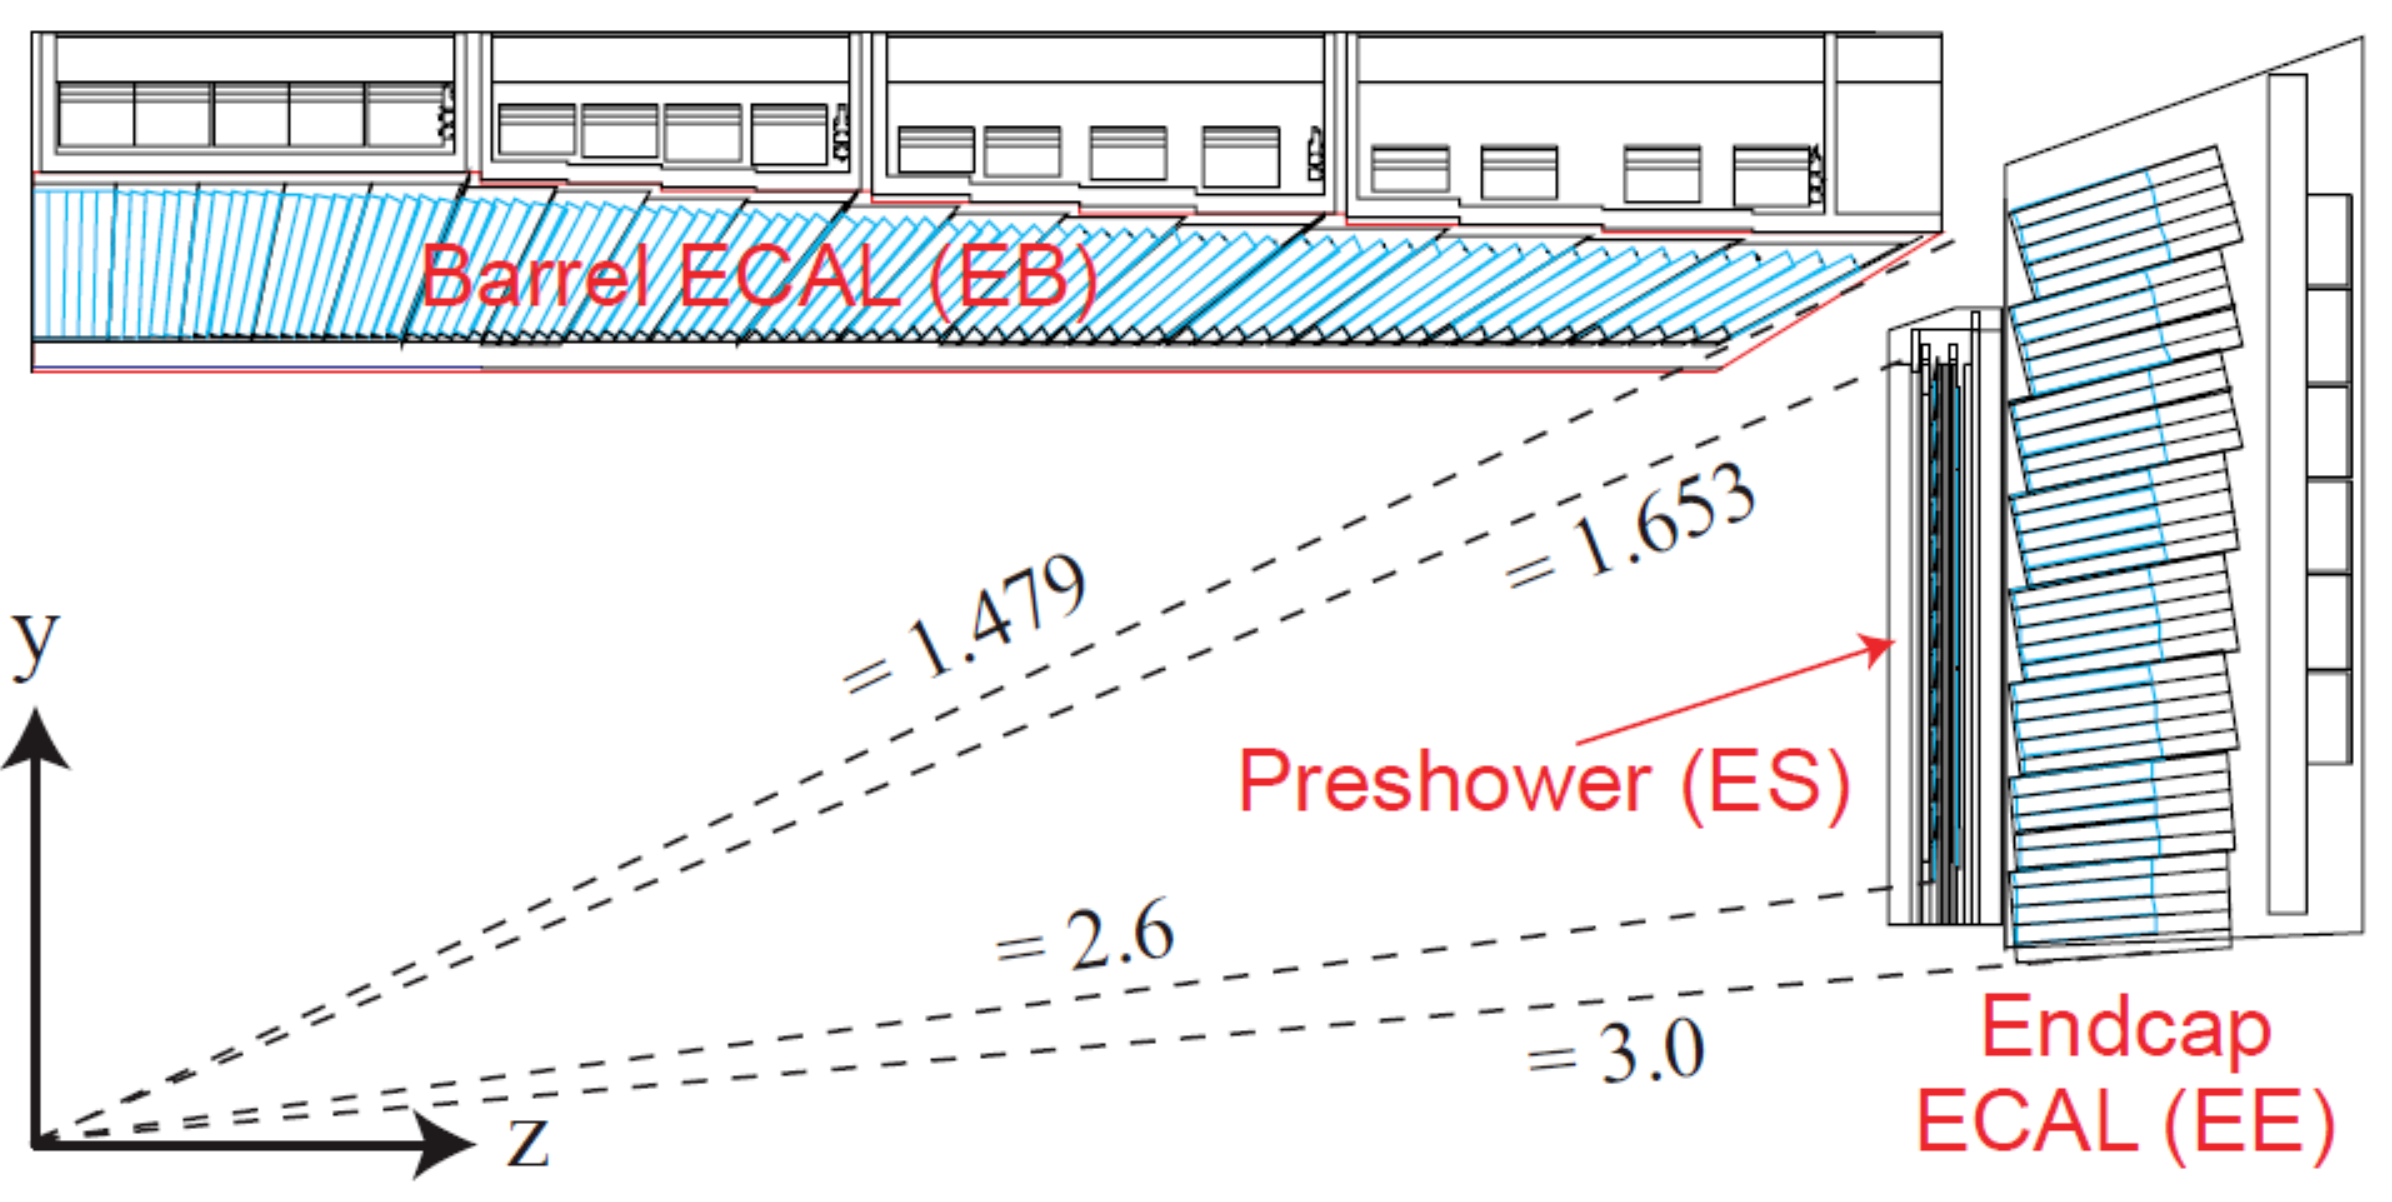
\includegraphics[width=\textwidth]{figs/ecal.png}
\caption{Diagram of the ECAL layout, emphasizing the crystal orientation. A small gap in the $\eta$ coverage is seen.}
\label{fig:ecal}
\end{subfigure}
\caption{The CMS electromagnetic calorimeter.}
\end{figure}

\subsection{Preshower}

The preshower is a more finely segmented region of the electromagnetic calorimeter intended for greater spatial resolution for resolving electromagnetic showers. It consists of two alternating layers of lead absorber and Si detectors (like the tracker) which are able to reconstruct the electron-positron pairs created at an early stage in the showering process. The silicon detector is able to reconstruct the electron and positron trajectories allowing for the greater spatial resolution compared to the rest of the calorimeter.

The preshower is designed to properly identify photon pairs resulting from high-$p_{T}$ neutral pion decay (98.8\% branching fraction). When a sufficiently high $p_{T}$ pion decays, the daughter photons become collimated to the extent they can not be separately resolved within the ECAL. Proper identification is crucial as neutral pions are one of the most copiously produced particles in these collisions. Preshower instrumentation only exists in a forward region $1.7<\eta<2.6$ where this poses the greatest challenge because of the pion kinematics.

\section{Hadronic Calorimeter}

The hadronic calorimeter is responsible for the reconstruction of hadrons: pions $\pi^{\pm}$, protons $p^{\pm}$, neutrons n, and kaons $K^{\pm}, K^{0}$. The particle energy is measured by collecting light generated by a hadronic shower as the particle is absorbed in the calorimeter.\cite{hcaltdr}

The bulk of the calorimeter consists of steel or brass absorber. A particle will interact with the material causing a shower of a number of secondary particles. These secondary particles in turn interact and this process creates a particle shower within the detector.  Interspaced with the absorber are tiles of clear plastic scintillator which create flashes of light after de-excitation of the scintillating molecules embedded in the plastic. Fibers are ran throughout the plastic and absorb the light, which is then piped to hybrid photodiodes. Light incident on the photodiodes liberates electrons via the photoelectric effect which are then accelerated onto the surface of a silicon diode which further amplifies and digitizes the signal.

A diagram of the HCAL is seen in Figure \ref{fig:hcal}. It is divided into barrel ($|\eta|<1.2$), endcap ($1.2<|\eta|<3$), and forward regions ($3<|\eta|<5.2$), containing over 9000 readout channels in total. The absorber is over a meter thick, consisting of about 16 layers of 5cm brass plates and 1cm thick scintillator. This thickness of absorber is sufficient to contain over 98\% of the energy of incident particles. For improved resolution of late-starting showers, there is an additional section of calorimeter in the barrel region outside the magnet solenoid.

\begin{figure}[hb!]
\centering
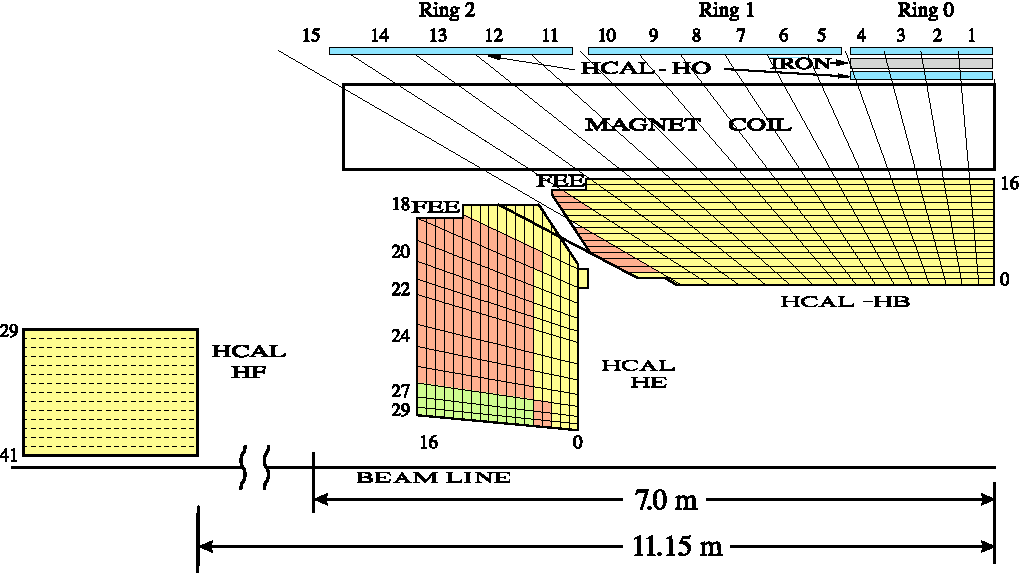
\includegraphics[width=0.8\textwidth]{figs/hcal.pdf}
\caption{The CMS hadron calorimeter. Color coding identifies optically summed channels.\cite{cosmichcal}}
\label{fig:hcal}
\end{figure}

\section{Solenoidal Magnet}

The CMS magnet provides the field necessary to deflect charged particles within the tracker to allow for a measurement of the momentum. The superconducting iron electromagnet delivers a uniform 3.8 T solenoidal field (parallel to the beampipe) within the silicon tracker volume. The magnetic field lines are returned via steel yokes sitting outside the magnet interspaced within the muon tracker volume, the field strength throughout the muon system is approximately 2 T.\cite{magnettdr}. A simulation of the magnetic field within the whole of CMS is seen in Figure \ref{fig:magnet} \cite{magnet}.

\begin{figure}[hb!]
\centering
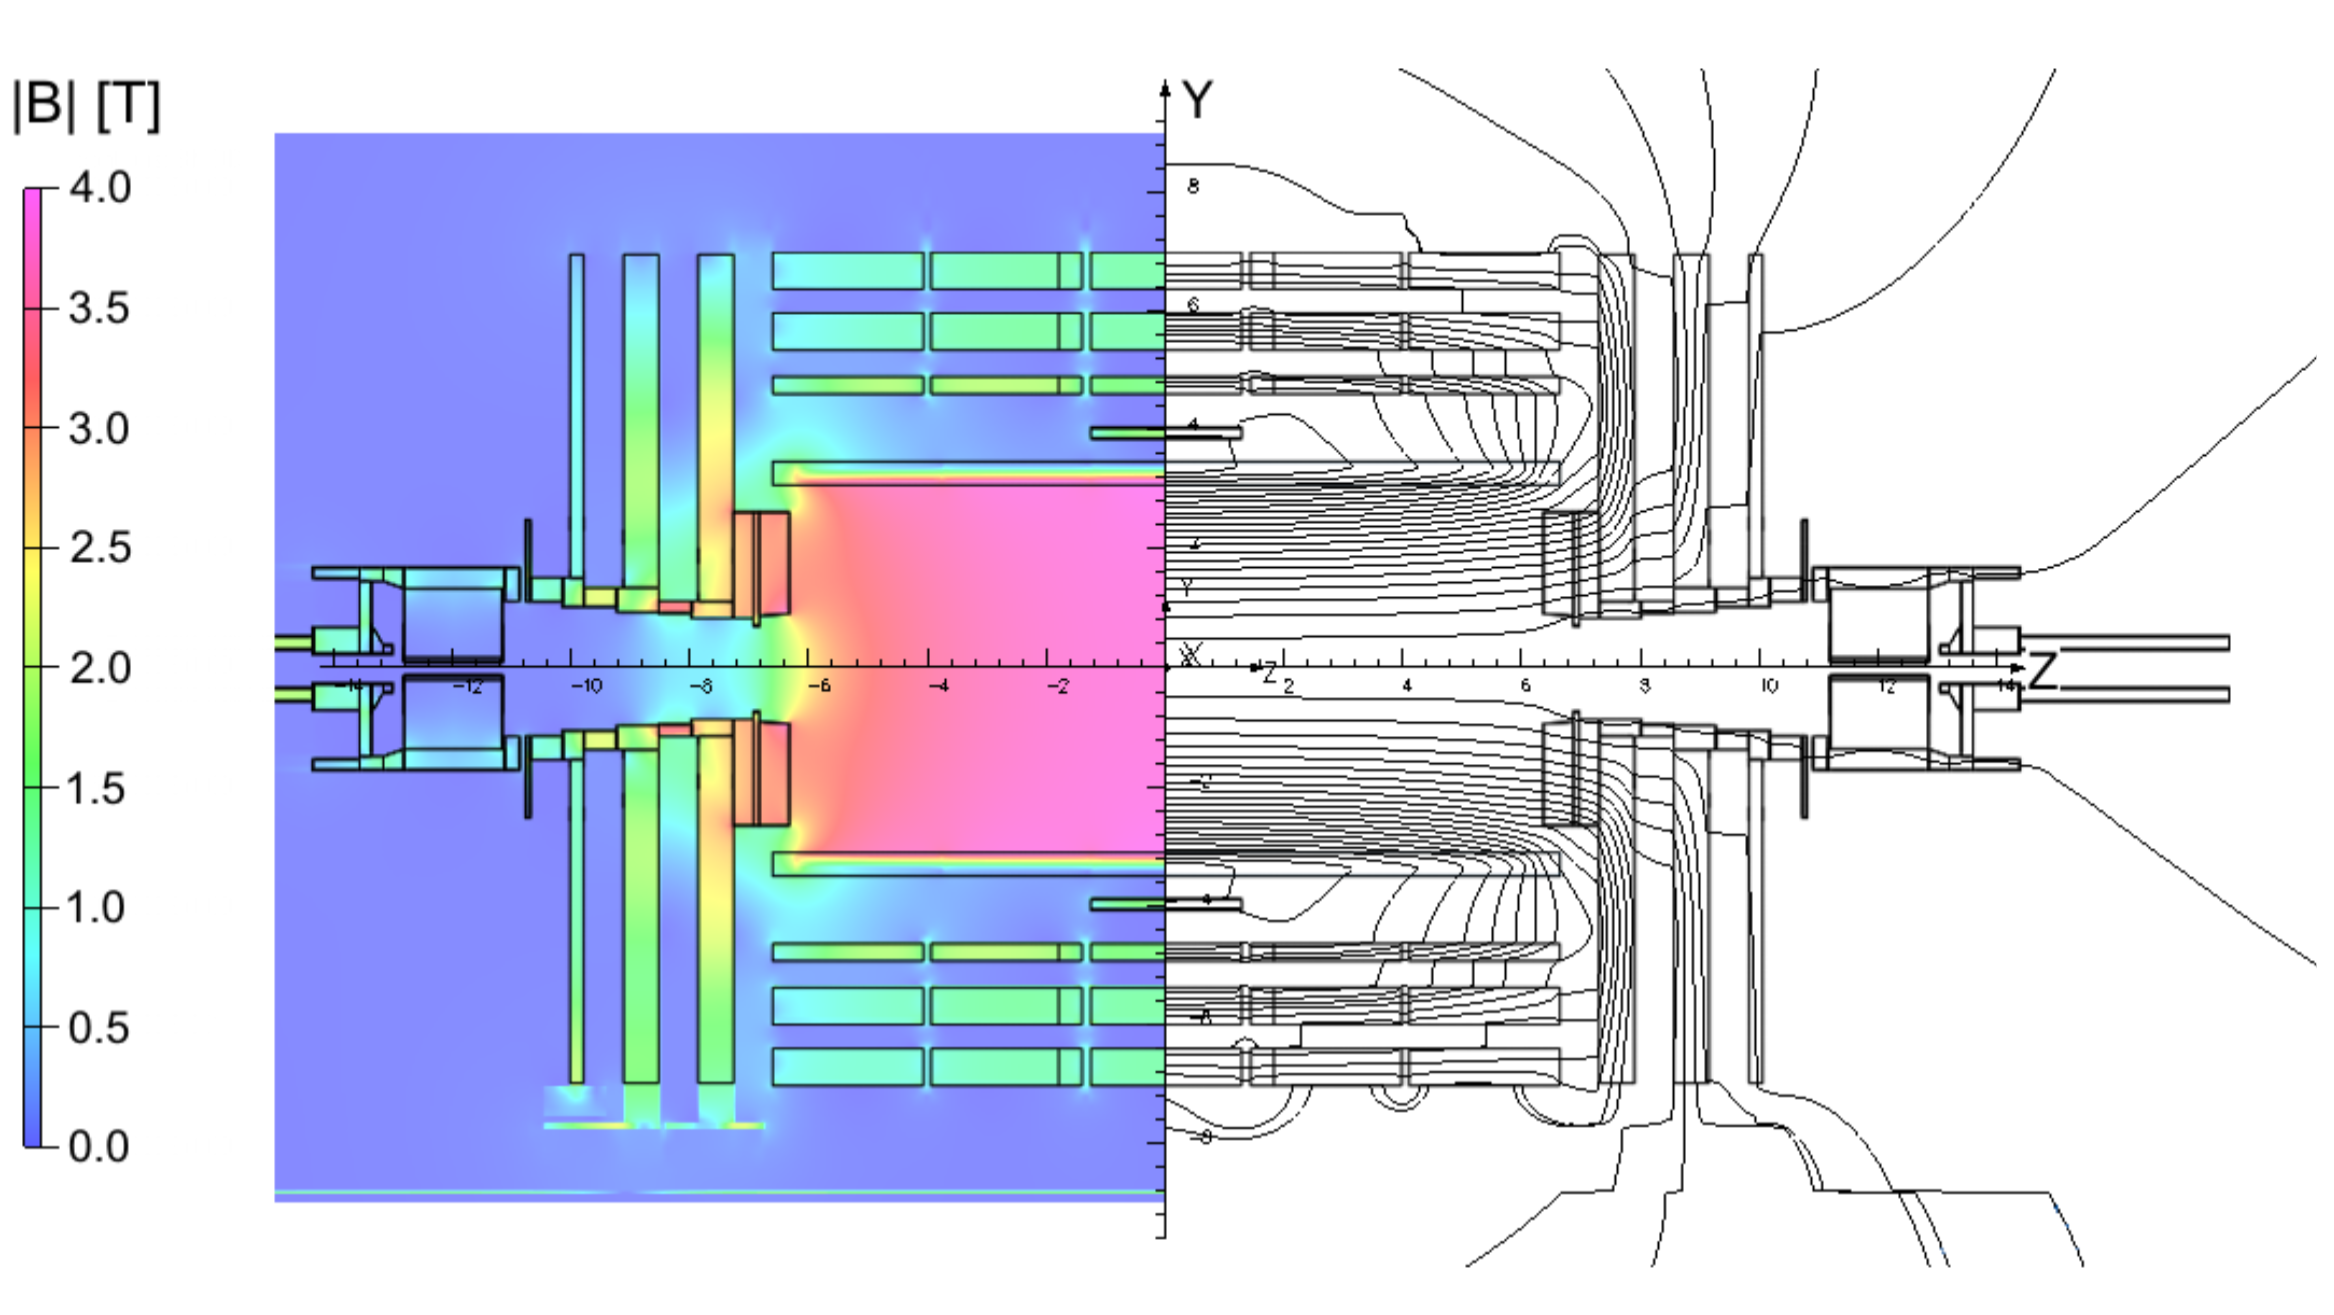
\includegraphics[width=0.7\textwidth]{figs/magnet.png}
\caption{A simulation of the magnetic field within CMS. The uniformity of the the 4T field within the tracker volume is crucial.}
\label{fig:magnet}
\end{figure}

\section{Muon System}

The muon system is responsible for the reconstruction (and triggering) of muons $\mu^{\pm}$. The muon trajectory is reconstructed using ionization deposits left in layers of gaseous detectors. The muon momentum is measured by the curvature of the trajectory when submerged in the magnetic field.\cite{muontdr}

The muon detectors sit at the furthest distance from the beamline, and any particles which have made the journey traveled through many layers of detector material (e.g. silicon Si, lead tungstate PbWO$_{4}$, brass (Cu), iron Fe) before being detected. Because of the relatively long lifetime and large mass of the muon they are the only particles which are expected to reach the muon detectors.

There are three components of the muon detector: drift tubes, cathode strip chambers, and resistive plate chambers. The drift tubes and cathode strip chambers are primarily used for tracking in the barrel and endcap regions, respectively. There is a small amount of overlap in coverage of the two subdetectors. The resistive plate chambers are used primarily for triggering and has coverage in the barrel and endcap regions, interspersed within the drift tubes and cathode strip chambers.

\subsection{Drift Tubes}

The drift tubes are used for muon tracking in the barrel portion of the detector ($|\eta|<1.3$). The basic element is a gas tube 4$\,$x$\,$1.3$\,$cm in transverse size and 2$\,$-$\,$4$\,$m long (depending on its position). High-voltage is applied to a wire strung the length of the cylinder and collects charge released when an incident muon ionizes the gas mixture. For economic and safety reasons the gas mixture is chosen to be Ar and CO$_{2}$. An 85/15\% fraction is chosen for nice gas quenching (shower avalanche) and drift velocity properties. \cite{dtperformance}

The drift tubes are divided into four barrel regions (each called a station) at different radii within the magnetic return yoke. Each station contains 3 \textit{superlayers}, where a superlayer is composed of four layers of stacked tubes, each layer staggered by one half width. For each station, two of the superlayers are oriented parallel to the beamline for $r-\phi$ measurements and one superlayer is perpendicular to the beamline to allow for measurements of the r-z position. An image of a DT station is seen in Figure \ref{fig:superlayer}.

\begin{figure}[hb!]
\centering
\begin{subfigure}[b]{0.475\textwidth}
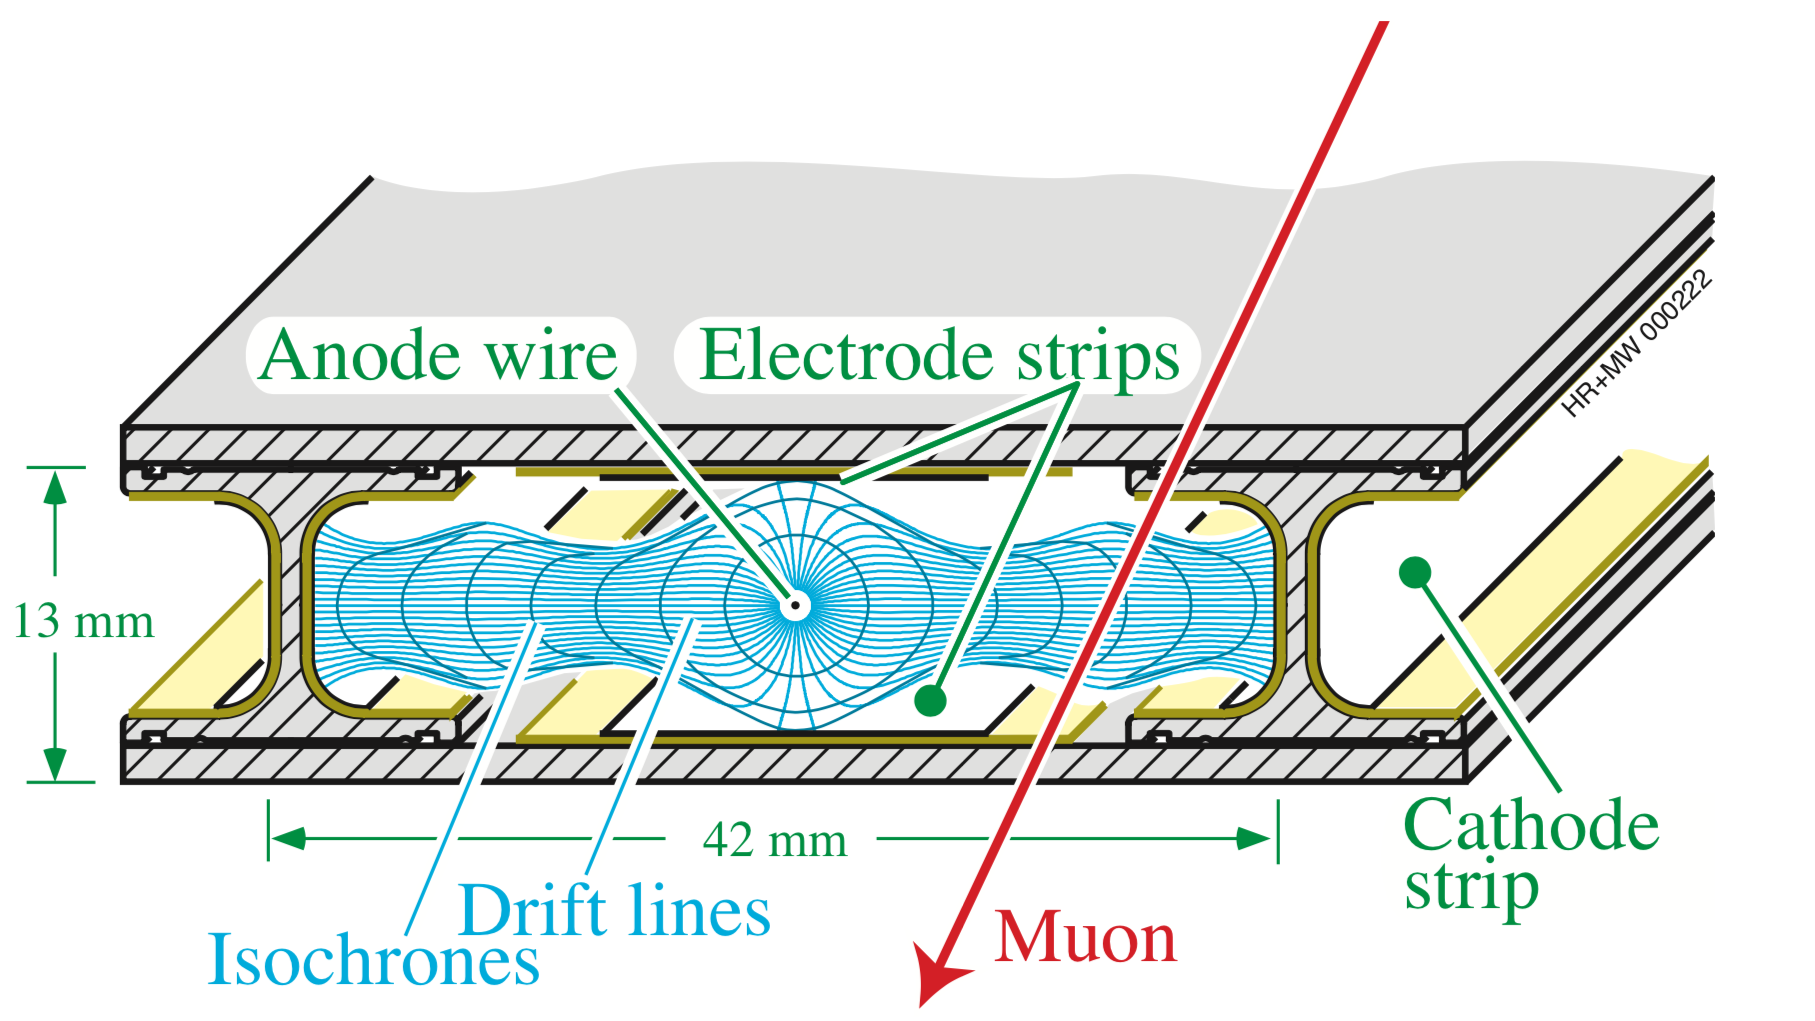
\includegraphics[width=\textwidth]{figs/dtcell.png}
\caption{Cross sectional view of a drift tube cell.}
\end{subfigure}
\begin{subfigure}[b]{0.475\textwidth}
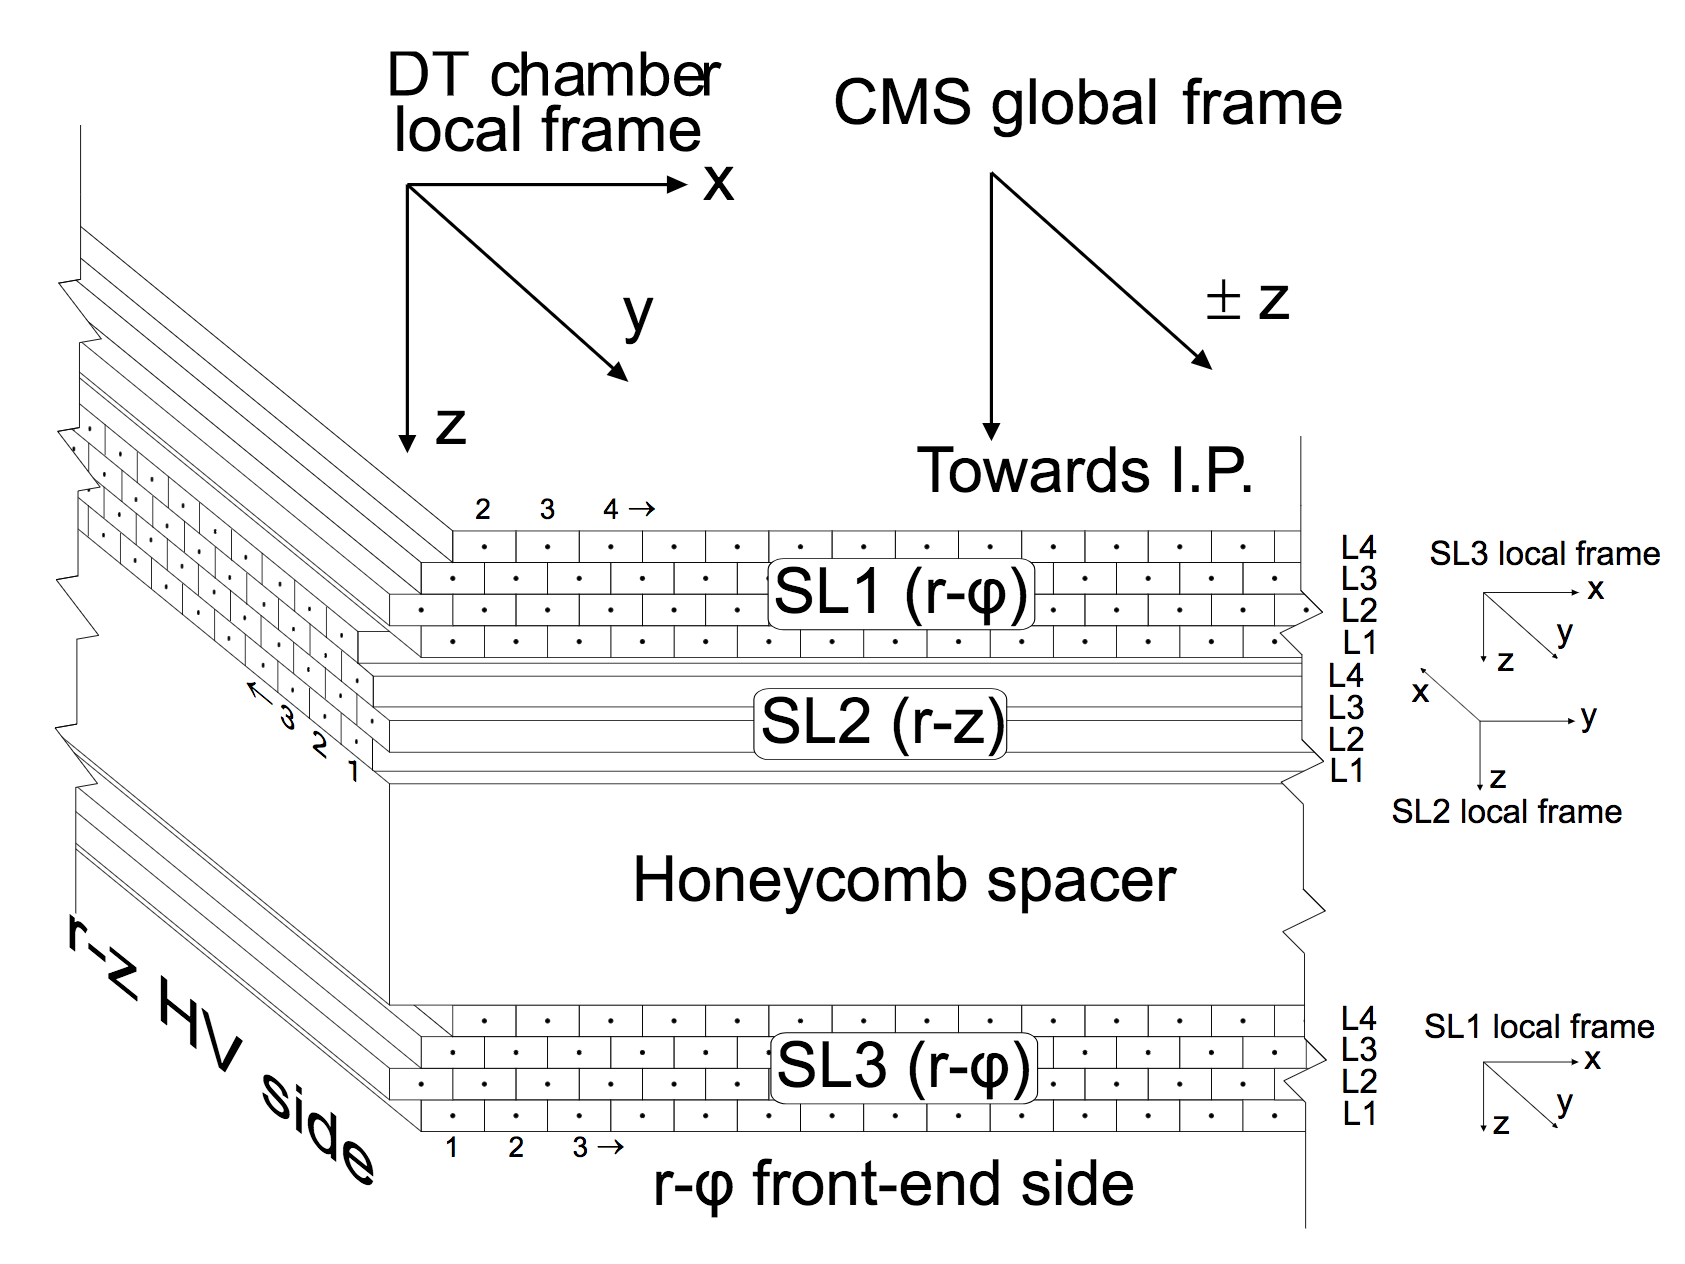
\includegraphics[width=\textwidth]{figs/superlayer.png}
\caption{Drift tube configuration within a superlayer.}
\end{subfigure}
\caption{The CMS muon drift tube detector.\cite{dtcellpic}}
\label{fig:superlayer}
\end{figure}

\subsection{Cathode Strip Chambers}

The cathode strip chambers are used for muon tracking in the endcap portion of the detector ($0.9<|\eta|<2.4$). The system is divided up into 468 trapezoidal chambers arranged in 2 or 3 concentric rings on a disk. There are 4 discs on either side of the detector ($\pm z$). The geometry of the chambers on a disk are seen in Figure \ref{fig:cscring} (an example image of the hit occupancy of a disc during cosmic ray runs). Each chamber (diagram in Figure \ref{fig:cscchamber}) consists of 6 layers of electrode planes separated by a gas layer of C$_{2}$H$_{2}$F$_{4}$ (freon) and C$_{4}$H$_{10}$ (isobutane). Wires are strung in the phi direction (concentric circles about the z axis) and therefore make a measurement of the radial coordinate of the hit. The electron shower generates an image charge in cathode planes. For each layer, one of the planes is segmented into strips which are perpendicular to the wires. Reading out the strips allows for additional hit information. The orientation of the strips is such that provides an additional measurement of the hit, a good measure of the $\phi$ coordinate. \cite{cscperformance}

\begin{figure}[hb!]
\centering
\begin{subfigure}[b]{0.55\textwidth}
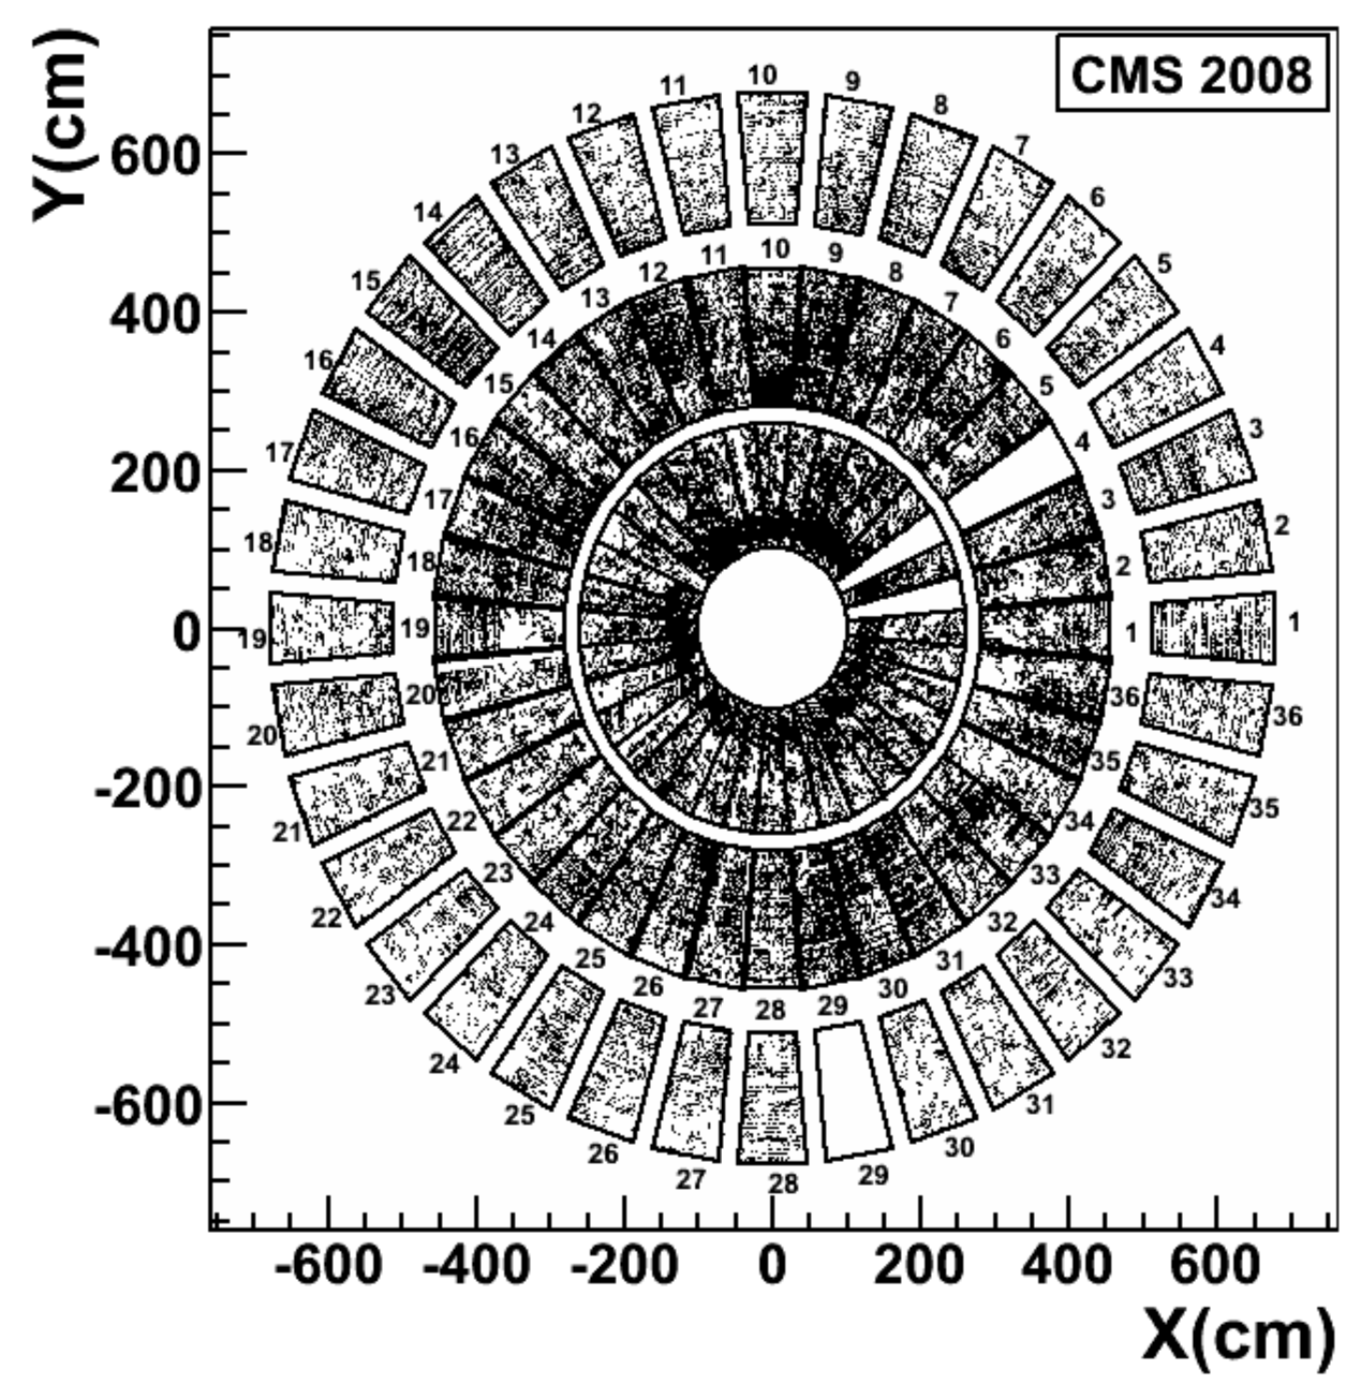
\includegraphics[width=0.8\textwidth]{figs/cscring.png}
\caption{Hit occupancy on one disc.}
\label{fig:cscring}
\end{subfigure}
\begin{subfigure}[b]{0.3\textwidth}
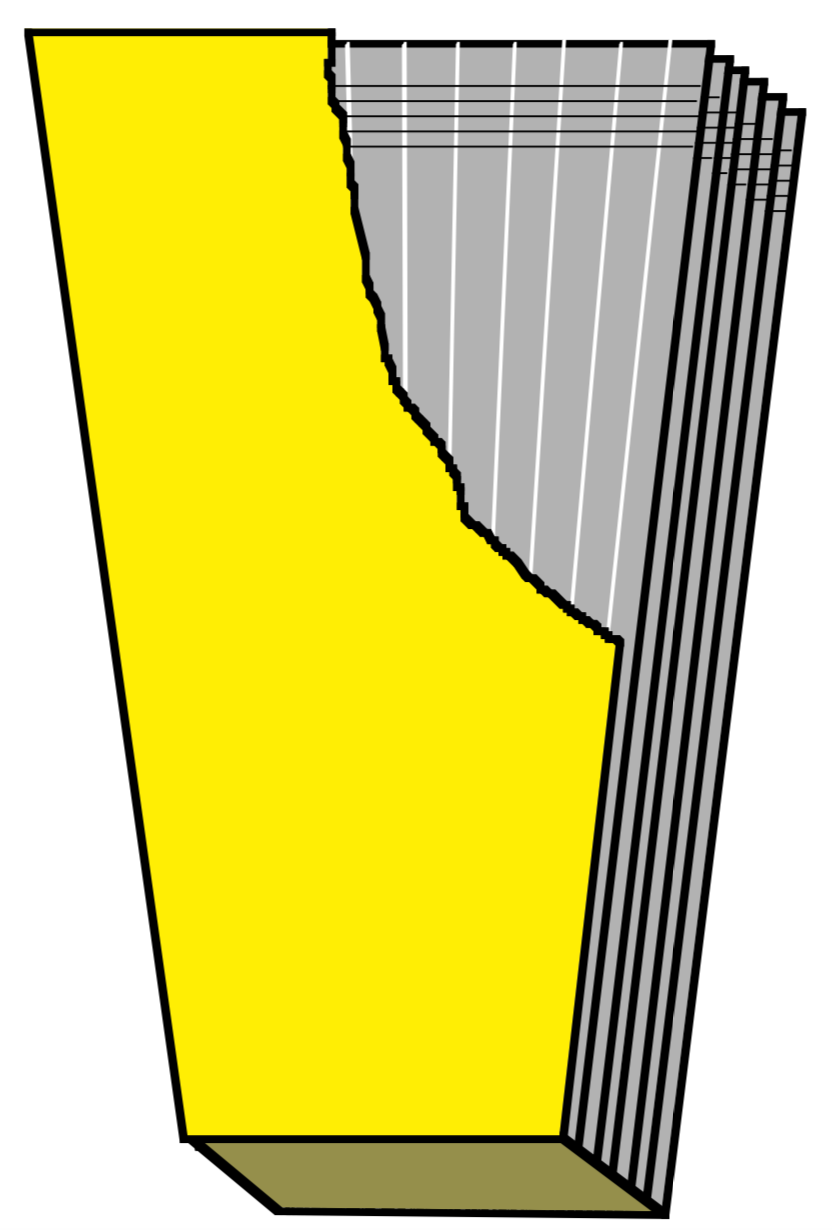
\includegraphics[width=0.9\textwidth]{figs/cscchamber.png}
\caption{One chamber - strips/wires are oriented vertically/horizontally.}
\label{fig:cscchamber}
\end{subfigure}
\caption{The CMS muon cathode strip chambers.}
\end{figure}

\subsection{Resistive Plate Chambers}

Resistive plate chambers cover the entire region within $|\eta|<2.5$ and are interspersed within the other muon detectors and the magnetic return yoke. They have an excellent timing resolution of about 3ns which allows for fast muon triggering and identification of the different bunch crossings. Pattern matching across the hits in the different layers allows for estimates of the muon $p_{T}$ to be used in further trigger processing. Hits created in the resistive plate chambers are additionally used for global fitting of the muon tracks.

The resistive plate chambers consist of an airtight system of two parallel high-resistivity planes separated by a 1cm gas gap. The outside of each plate is coated to form an electrode for the high-voltage bias. On top of each electrode sits aluminum strips which are insulated from the electrode and serve as the readout. Electron showers created in the gas bulk induce an image charge on the strips which is then recorded.

\section{Trigger System}

While in operation mode, the LHC provides collisions at a rate of 400 MHz (25ns per bunchcrossing). This is a phenomenal rate which the CMS detector bandwidth is not able to accommodate, nor does the experiment have access to the amount of disc space necessary to store all this information. Therefore, the CMS detector makes use of a trigger system to quickly determine if the event is 'interesting' and will be saved for storage - events which are not triggered are lost forever. Examples of interesting events contain those with high-$p_{T}$ muons, or a large imbalance in the total momentum of the event.\cite{CMS-TRG-12-001}

The trigger consists of two stages known as the Level-1 (L1) and High-Level Trigger (HLT). L1 is a hardware based trigger which combines information from the calorimeters and muon systems to make a decision if the event will be passed to HLT for further processing. L1 is able to reduce the event rate from 400 MHz to 100 kHz and must make the decision within $4\,\mu s$. Primitive objects such as calorimeter energy deposits or muon track segments are first constructed locally within the detector before being combined to form the global decision at L1. The flowchart seen in Figure \ref{fig:trigger} illustrates the L1 system. If the decision is made at L1 that the event is of potential interest, it is passed to HLT. HLT is a software based trigger which makes use of more sophisticated reconstruction algorithms which can be tuned to select events of choice.

\begin{figure}[hb!]
\centering
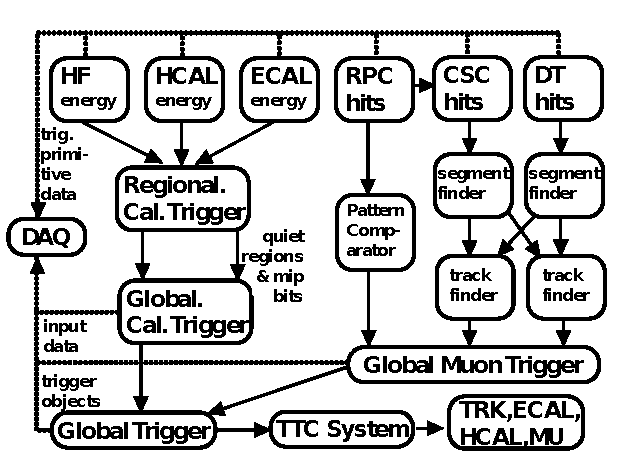
\includegraphics[width=0.6\textwidth]{figs/CMS-TRG-12-001_Figure_002.pdf}
\caption{The CMS L1 trigger system; trigger logic flows from local (top) to global (bottom).}
\label{fig:trigger}
\end{figure}
